\documentclass[20 pt, a0paper, portrait]{tikzposter}
\usepackage[utf8]{inputenc}
\usepackage{amsmath}
\usepackage{amssymb}
\usepackage{doi}
\hypersetup{
    colorlinks=true,
    citecolor=black,   
    urlcolor=cyan,
}
 
\urlstyle{same}

\geometry{paperwidth=24in,paperheight=36in}
\makeatletter
\setlength{\TP@visibletextwidth}{\textwidth-2\TP@innermargin}
\setlength{\TP@visibletextheight}{\textheight-2\TP@innermargin}
\makeatother

\title{Fourth Order Modified Laguerre's Method}
\author{Thomas R. Cameron}
\date{\today}
\institute{Mathematics and Computer Science Department, Davidson College}
 
\usepackage{blindtext}
\usepackage{comment}

\usetheme{Autum}
 
\begin{document}
 
\maketitle

%%%%%%%%%%%%%%%%%%%%%%%%%%%%%%%%%%%%%%%%
%								Abstract						%
%%%%%%%%%%%%%%%%%%%%%%%%%%%%%%%%%%%%%%%%
\block{Abstract}
{
We present a novel modification of Laguerre's method that results in a method for the concurrent approximation of all roots of a univariate polynomial. Our method has strong virtues including fourth-order convergence that is observed in practice and belonging to the class of embarrassingly parallel algorithms. A Fortran 90 implementation of our algorithm is available online and comparisons with several other software are provided. 
}

\begin{columns}
	\column{0.6}
	%%%%%%%%%%%%%%%%%%%%%%%%%%%%%%%%%%%%%%%%
	%							The Algorithm						%
	%%%%%%%%%%%%%%%%%%%%%%%%%%%%%%%%%%%%%%%%
	\block{The Algorithm}
	{
		Let $p(\lambda)=a_{0}+a_{1}\lambda+\cdots+a_{m}\lambda^{m}$ be a polynomial with $a_{0}a_{m}\neq 0$ and denote by $(z_{1},\ldots,z_{m})$ the current approximations to the roots of $p(\lambda)$. The $j$th approximation is updated via
		\begin{equation}
		\hat{z}_{j}=z_{j}-\frac{m}{G_{j}\pm\sqrt{(m-1)(mH_{j}-G_{j}^{2})}},
		\end{equation}
		where 
		\begin{equation}
		G_{j}=\frac{p^{'}(z_{j})}{p(z_{j})}-\sum_{\substack{i=1\\i\neq j}}^{m}\frac{1}{(z_{j}-z_{i})}~\text{ and }~H_{j}=-\left(\frac{p^{'}(z_{j})}{p(z_{j})}\right)^{'}-\sum_{\substack{i=1\\i\neq j}}^{m}\frac{1}{(z_{j}-z_{i})^{2}}.
		\end{equation}
		On each iteration, $z_{j}$ is updated for $j=1,\ldots,m$, unless it was accepted on a previous iteration.
		
	\textbf{Initial Estimates.} In essence, we select complex numbers along circles of suitable radii. What constitutes suitable radii is formalized in~\cite{Bini1996} and can be computed via the upper envelope of the convex hull of the set $\{(i,\log|a_{i}|),~i=0,1,\ldots,m\}$. We compute the convex hull via Andrew's Monotone Chain algorithm~\cite{Andrew1979}.
	
	\textbf{Backward Error.} The backward error of an approximate root $\xi$ is given by
	\begin{equation}
	\eta(\xi)=\frac{|p(\xi)|}{\alpha(\xi)},
	\end{equation}
	where $\alpha(\xi) = \sum_{i=0}^{m}|e_{i}||\xi|^{i}$ and $e_{i}$ represent tolerances against which perturbations are measured. We accept a root approximation $\xi$ if $\eta(\xi)<\mu$, where $\mu$ is machine precision. 
	
	\textbf{Condition.} The condition of a nonzero approximate root $\xi$ is given by
	\begin{equation}
	\kappa(\xi)=\frac{\alpha(\xi)}{|\xi||p^{'}(\xi)|}.
	\end{equation}
	If the root approximation $\xi$ is accepted, then we also return its condition.
	}
	%%%%%%%%%%%%%%%%%%%%%%%%%%%%%%%%%%%%%%%%
	%							Numerical Experiments				%
	%%%%%%%%%%%%%%%%%%%%%%%%%%%%%%%%%%%%%%%%
	\block{Numerical Experiments}
	{
	Comparisons between FPML, Polzeros~\cite{Bini1996}, and the singleshift version of AMVW~\cite{Aurentz2015}.
	\vspace*{-2em}
	\begin{center}
	\begin{tabular}{ p{12cm} p{12cm}}
		\begin{tikzfigure}[Random Polynomials]
		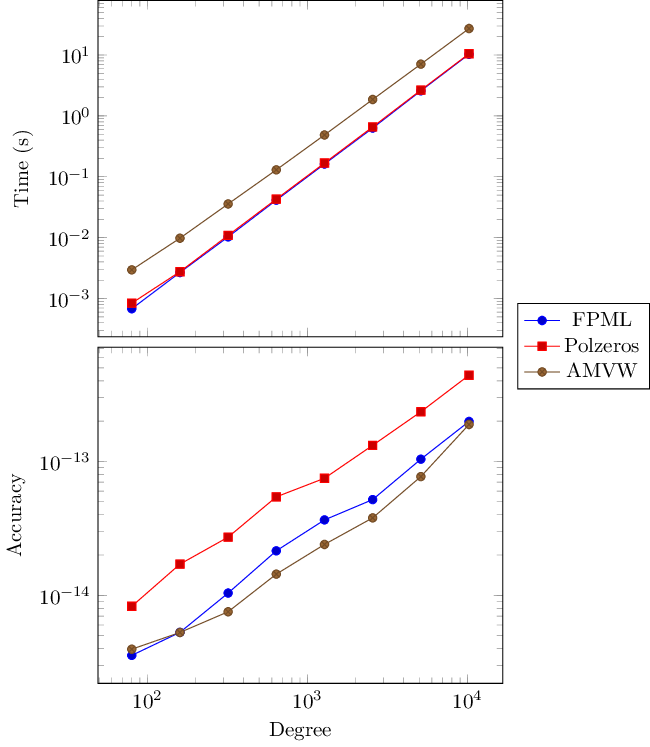
\includegraphics[scale=0.44]{../tests/figures/rand_poly.png}
		\end{tikzfigure}
		&
		\begin{tikzfigure}[Roots of Unity]
		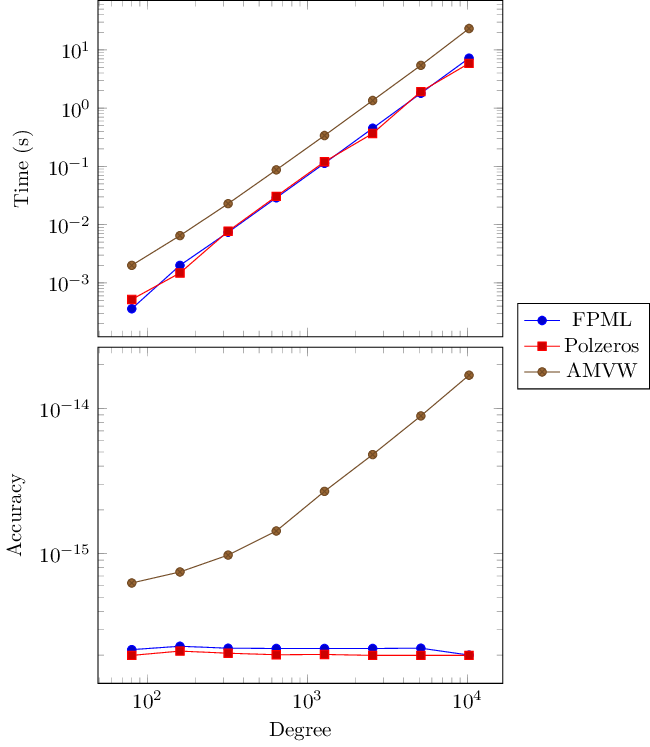
\includegraphics[scale=0.44]{../tests/figures/unity.png}
		\end{tikzfigure}
	\end{tabular}
	\vspace*{-2em}
	\begin{tikzfigure}[Special Polynomials]
		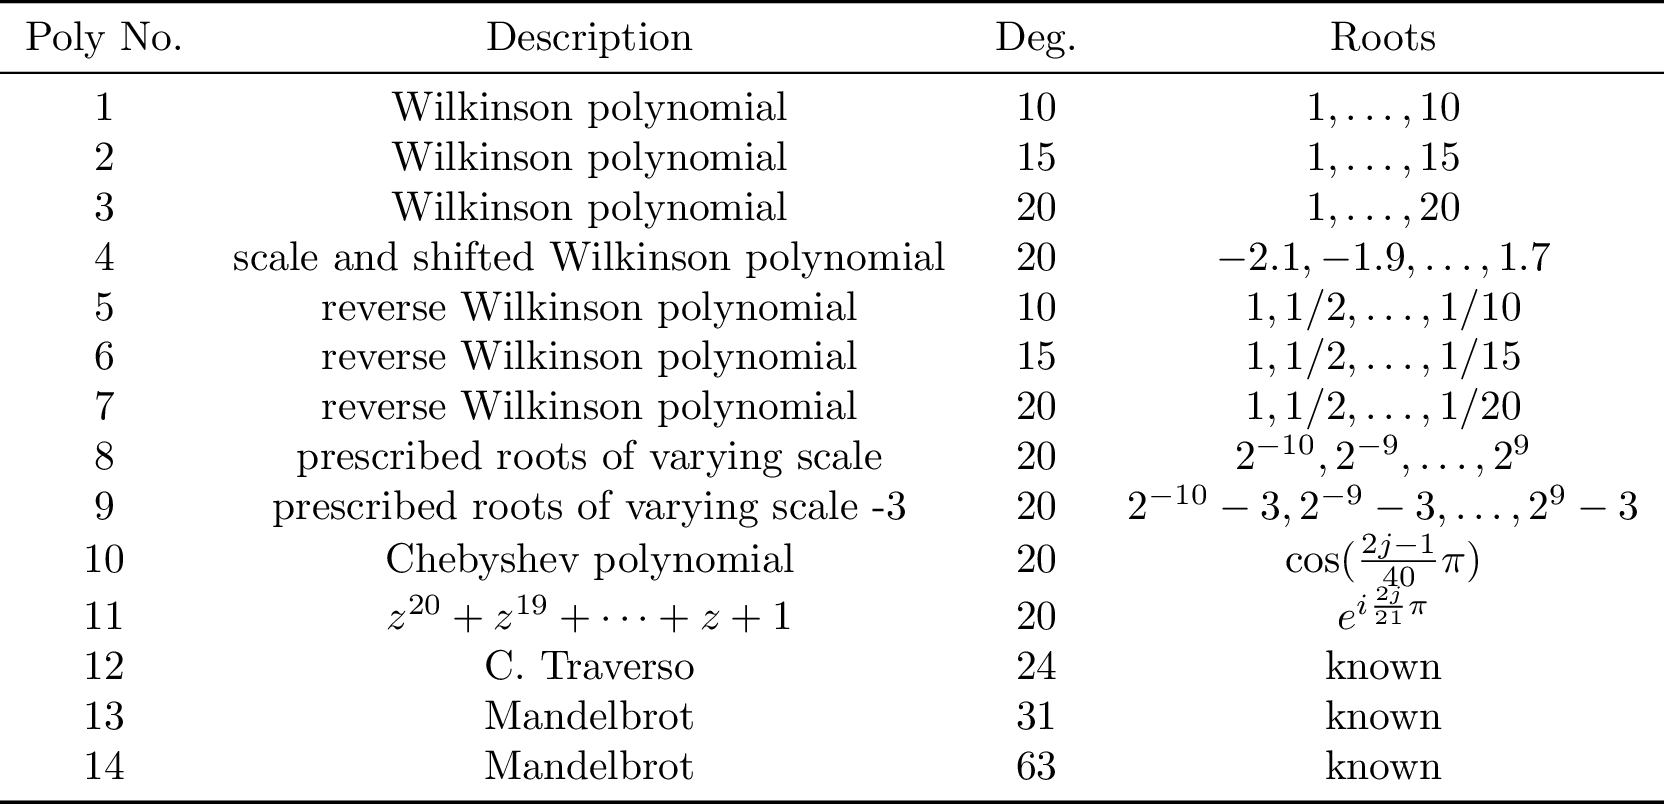
\includegraphics[scale=0.26]{../tests/figures/spec_poly_list.png}
		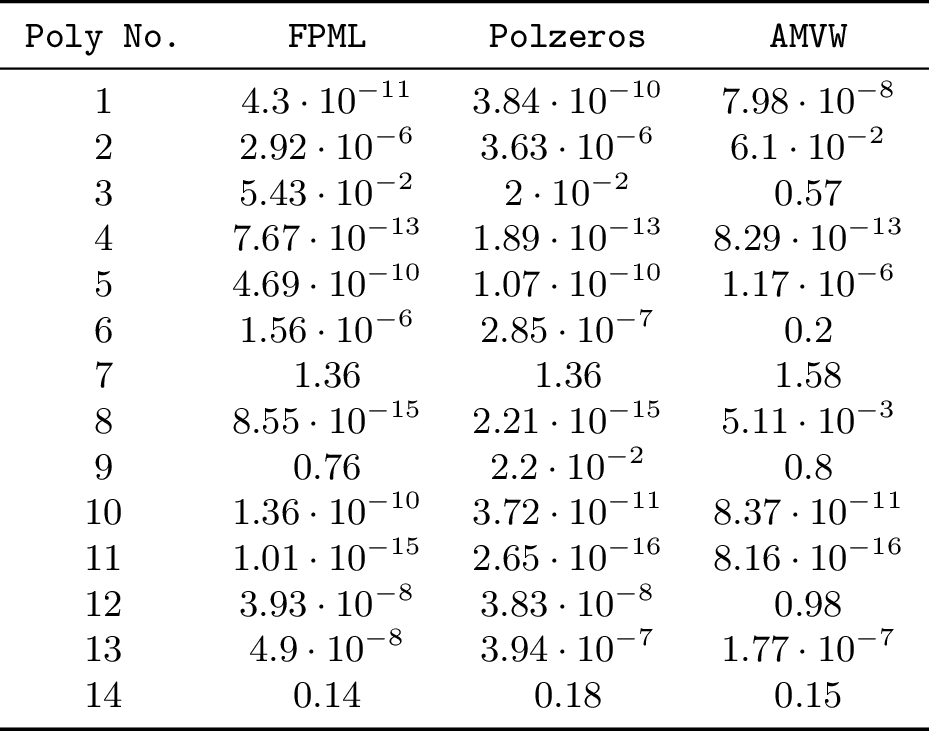
\includegraphics[scale=0.41]{../tests/figures/spec_poly_results.png}
		\end{tikzfigure}
	\end{center}
	}
	
	\column{0.4}
	%%%%%%%%%%%%%%%%%%%%%%%%%%%%%%%%%%%%%%%%
	%							Examples							%
	%%%%%%%%%%%%%%%%%%%%%%%%%%%%%%%%%%%%%%%%
	\block{Examples}
	{
	\textbf{Initial Estimates.} Let
	\[
	p(\lambda)=1+3\cdot10^{3}\lambda+3\cdot10^{6}\lambda^{2}+1\cdot10^{9}\lambda^{9}+\lambda^{10}.
	\] 
	The initial estimates and exact roots of $p$ are below.
	\begin{tikzfigure}
	\centering
	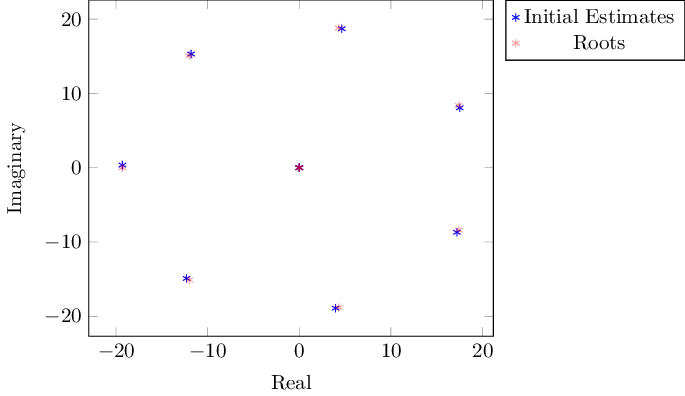
\includegraphics[scale=0.85]{../tests/figures/init_est_acc.png}
	\end{tikzfigure}
	
	\textbf{Convergence.} Here we test the convergence of the roots of three polynomials. The first polynomial is $z^{5}-1$, the second is the degree $10$ Chebyshev polynomial, and the third is $z^{10}+\cdots+z+1$. The error is measured as the maximum relative forward error. For each polynomial, the error after each iteration is recorded in the table below.
	\vspace*{-2em}
	\begin{tikzfigure}
	\centering
	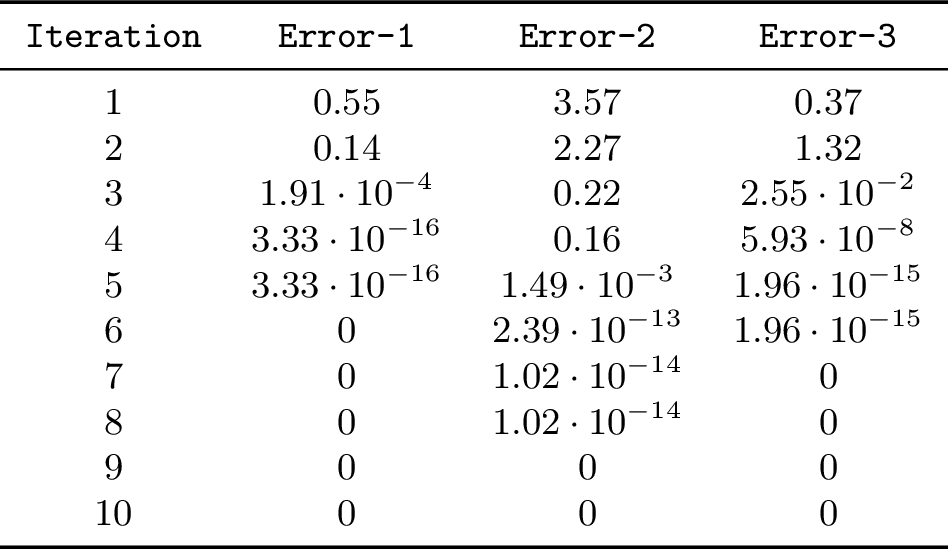
\includegraphics[scale=0.60]{../tests/figures/conv.png}
	\end{tikzfigure}
	}
	%%%%%%%%%%%%%%%%%%%%%%%%%%%%%%%%%%%%%%%%
	%							Conclusion						%
	%%%%%%%%%%%%%%%%%%%%%%%%%%%%%%%%%%%%%%%%
	\block{Conclusion}
	{
	Fortran 90 code along with installation instructions and additional experiment results and references are provided at \url{https://github.com/trcameron/FPML}.
	\vspace*{-1em}
	\bibliographystyle{amsplain}
	\bibliography{Bibliography}
	}
 \end{columns}
 
\end{document}